近年、様々なビデオ会議アプリケーション(図\ref{fig:1})が登場している。
その例としては、zoom\cite{1}やGoogle Meet\cite{2}が挙げられる。

\begin{figure}[tp]
  \centering
  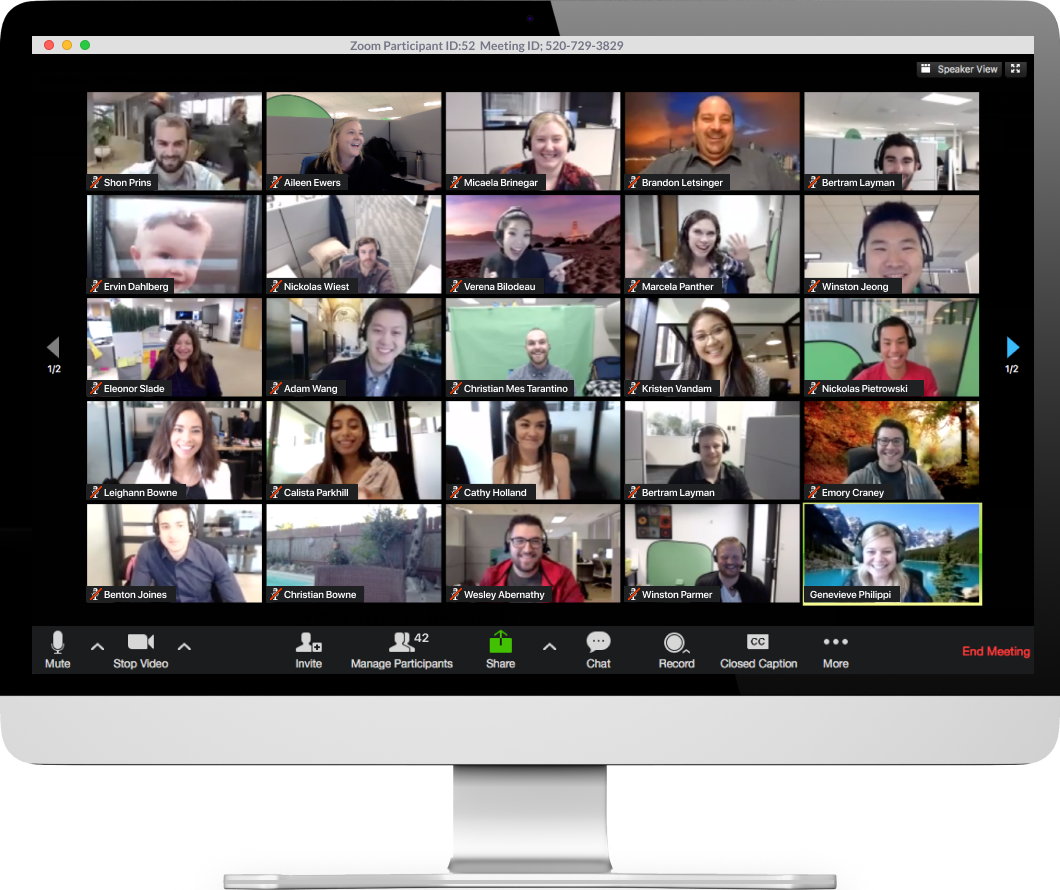
\includegraphics[scale=0.5]{fig/zoom-monitor-screen.png}
  \caption{zoom}\label{fig:1}\cite{1}
\end{figure}

90年代から2000年にかけてビデオ通話や遠隔会議システムが出てきた.
2020年は,新型コロナウイルス感染症の流行により,遠隔会議の需要が
さらに高まっている.遠隔会議の形態は様々であり,例えば以下のようなものが考えられる.
\begin{itemize}
  \item 個人間を結ぶ通信
  \item 同じ空間にいる複数人と,遠隔地の参加者の通信
  \item 複数人のグループ間での通信
\end{itemize}

1つ目は最も一般的な場合である.2つ目は,例えばある病に感染するなどで
他の人物と接触できない人物が,グループの会話に参加する場合などに考えられる.
3つ目は,異なる研究室間のミーティング等が行われる場合である.

\begin{figure}[tp]
  \centering
  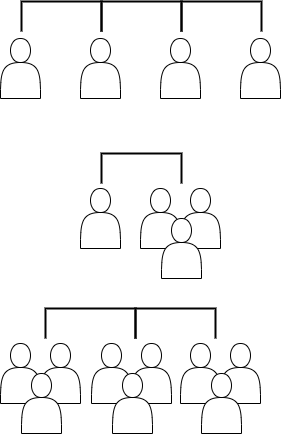
\includegraphics[scale=0.7]{fig/conference.png}
  \caption{遠隔会議の様式}
\end{figure}

しかし,ビデオ会議における様々な問題点も指摘されている。
例えばRoel\cite{3}は、カメラの視覚外の情報や,人物の情報の不足のために、対面時のような
インタラクションを得られないことを指摘している。

一方で,昨今は誰でも気軽に全天球映像(図\ref{fig:2})を撮影することができるようになっている,
その例として,全天球カメラ(360度カメラ,全天周カメラ,全方位カメラなどともいう (図\ref{fig:3}))
を使用して,全天球映像をヘッドマウントディスプレイを用いて観覧したり,パノラマ映像として動画や静止画を
保存することが出来るようになっている.
\begin{figure}[tp]
  \centering
  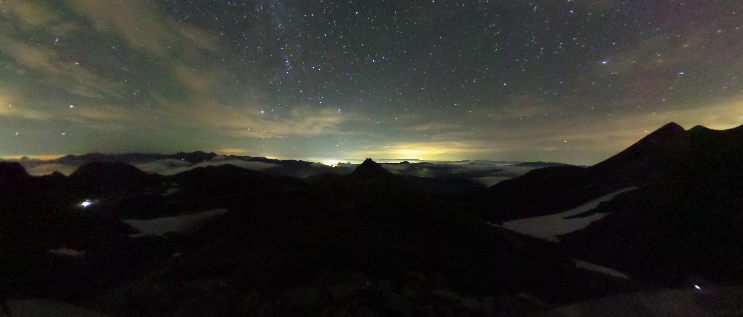
\includegraphics[scale=0.6]{fig/panorama.png}
  \caption{全天球パノラマ画像}\label{fig:2}\cite{4}
\end{figure}
\begin{figure}[tp]
  \centering
  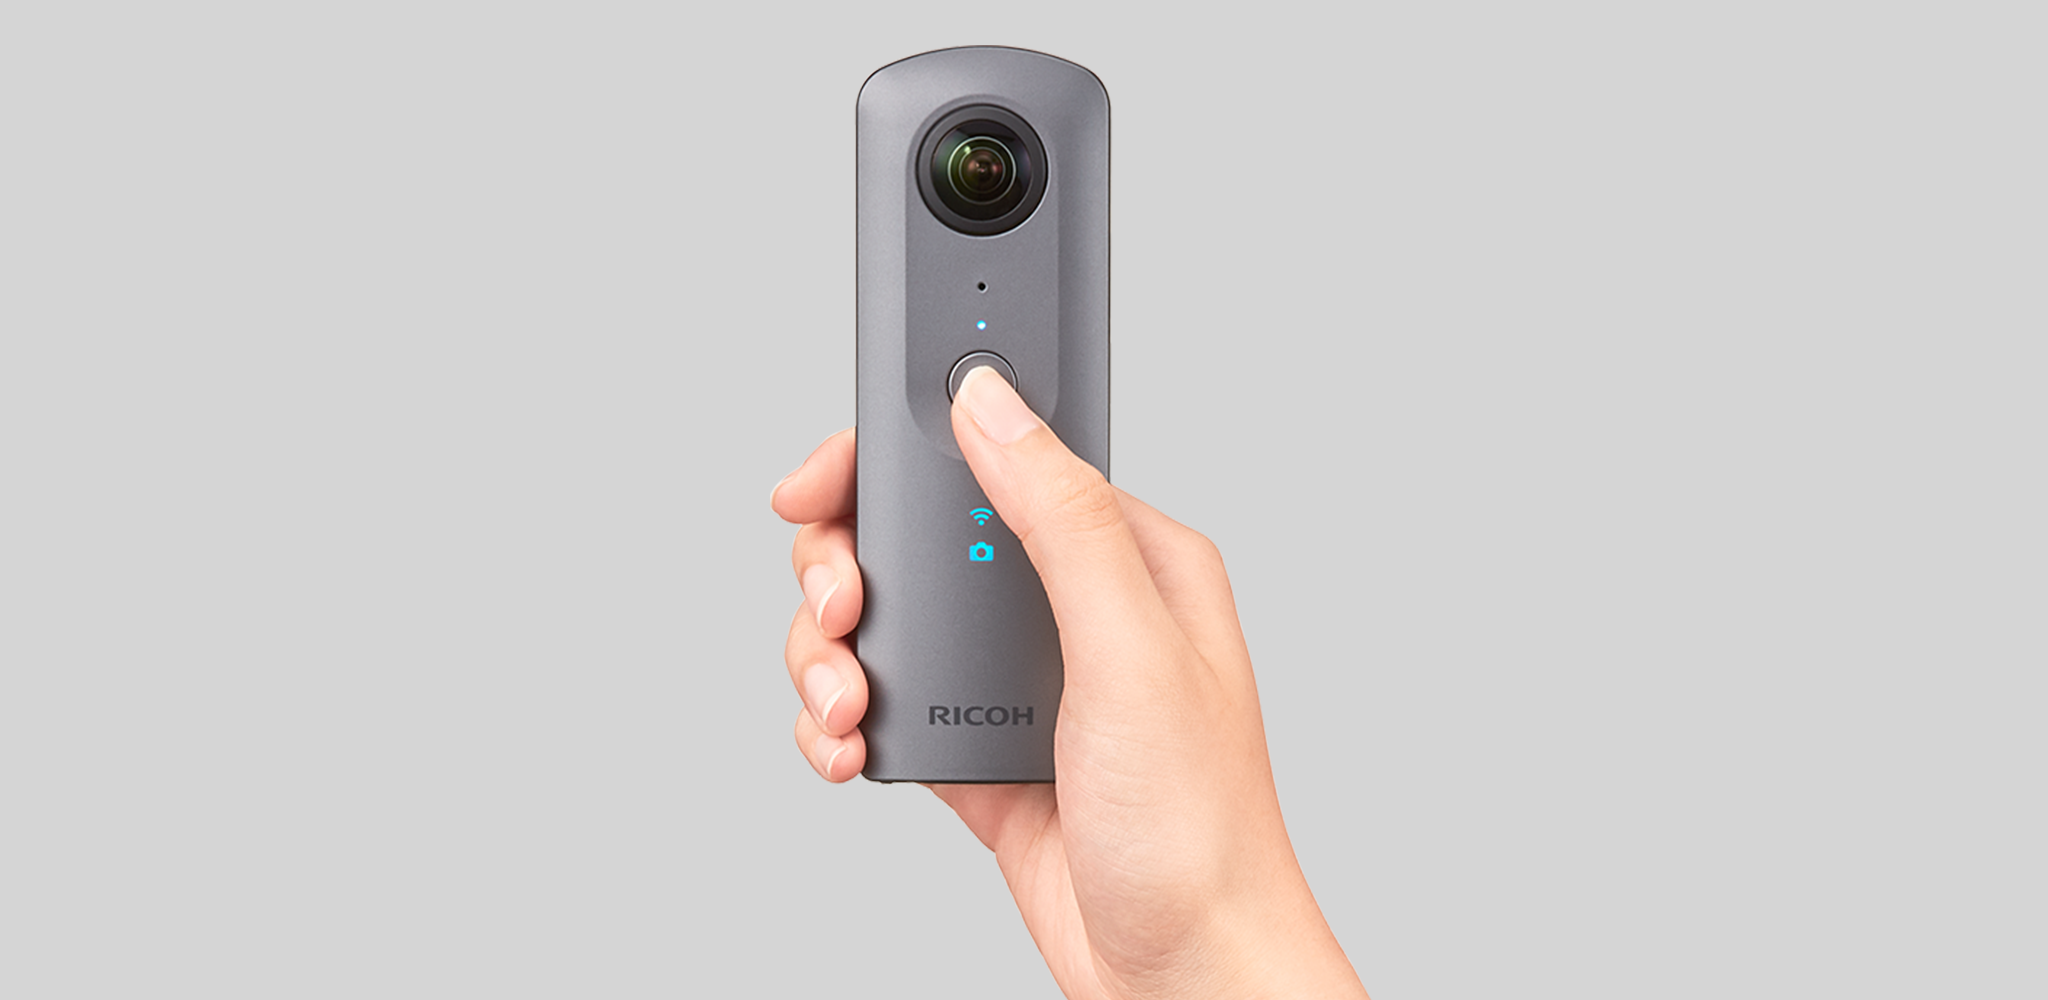
\includegraphics[scale=0.2]{fig/thetaV.png}
  \caption{theta V}\label{fig:3}\cite{4}
\end{figure}

全天周カメラの使用により,カメラの視野の問題は解決される.
実際に,Anthonyら\cite{5}は,全天球の視野の広さによって,リモートユーザーが
ローカルユーザーの環境をより早く理解できると結論付けている.
だが、Johnsonら\cite{6}によって,パノラマ視野によって映像の複雑さが増し、
より大きな認知負荷を必要としたことも示されている.加えてTangら\cite{19}は,
全天球カメラの使用者がどこを見ているかを知る手段が無ければ,コミュニケーションが
困難になることを報告している.

認知負荷を削減するため、パノラマ映像を3次元に表示する、球体プロジェクター\cite{15}を
用いた方法が挙げられる。球体プロジェクターの利用としては、LiらのOmniEyeBall\cite{18}\cite{24}
がある.OmniEyeBallを用いた実験では,平面ディスプレイによるパノラマ映像の表示
より,球体ディスプレイによるの表示の方が,歪みの低下,立体感の上昇
などから視覚認知が向上されたことが報告されている.

\begin{figure}[tp]
  \centering
  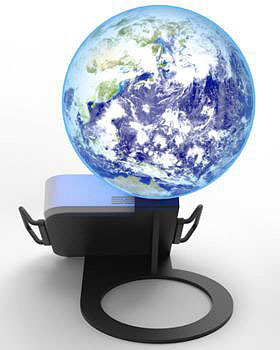
\includegraphics[scale=1.4]{fig/Glomal350.jpg}
  \caption{球体プロジェクター}\cite{15}
\end{figure}

